\chapter{Einleitung}
\label{sec:Chapter1}


Ziel dieses Praktikums war es zu erörtern, wie zwei Parteien die Ähnlichkeit ihrer DNA  berechnen können, ohne, dass dabei eine der Parteien Informationen über den genetischen Code der jeweils anderen erlangt.
Die Grundlagen für diese Berechnungen basieren auf bereits existierenden Methoden, mit welchen der Schnitt zweier Mengen unter Sicherung der Privatsphäre berechnet werden kann.
Im Zuge dieses Praktikums habe ich drei dieser Methoden mit Bezug zum gegebenen Anwendungsfall implementiert und deren Effizienz miteinander vergleichen:



\section{ Single nucliotide polymorphism (SNP)}

Da der Großteil der DNA bei allen Menschen identisch ist, ist es 
Um die DNA zweier Personen zu vergleichen, wurden nicht deren gesamte DNA Sequenzen  betrachtet, sondern lediglich die Unterschiede zwischen den Sequenzen.
Solche Unterschiede könne durch genetische Marker repräsentiert werden. Unter diesem werden bestimmte klar definierte Sequenzen und Positionen im genetischen Code bezeichnet, welche dazu genutzt werden können Individuen zu identifizieren.
\begin{figure}[htbp] 
	\centering
    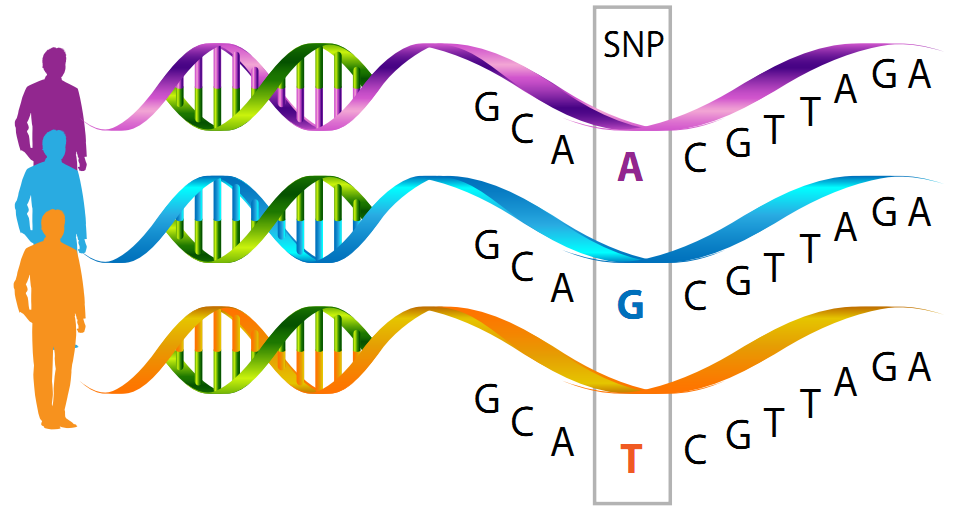
\includegraphics[width=0.7\textwidth]{./Graphics/snp.png}
	\caption{Schematische Darstellung eines Single nucleotide polymophism in drei Personen }
	\label{fig:Bild1}
\end{figure}


Für dieses Praktikum wurden Single Nuleotide Polymorphisms (SNPs) als  Marker gewählt.
Bei einem SNP handelt es sich um die Variation eines einzelnen Nuklotids an einer bestimmten Position in einem Genom im Verhältnis zu einem Referenzgenom. 

Diese Variationen treten mit unterschiedlichen Häufigkeiten auf. Während einige bei lediglich weit unter einem Prozent der Bevölkerung auftreten, sind andere deutlich weiter verbreitet. Diese etwas häufigeren und damit bekannteren SNPs.

Eine der größten Datenbanken mit über 149.000.000 SNPS ist die dbsnp.
Auf diese Datenbank wurde auch in diesem Praktikum zurückgegriffenen.
 
Die dbsnp wurde von dem National Center for biotechnological Information  1998 erstellt. Die NCBI sammelt für die dbsnp  Information aus diversen Quellen, wie Forschungslaboren, Sequenziereungszentren  und anderen Datenbanken und vereigit sie in einer einzigen.  Hierbei wird jedem Polymorphismus ein einzigartiger Code zugeordnet.
\begin{figure}[htbp] 
	\centering
	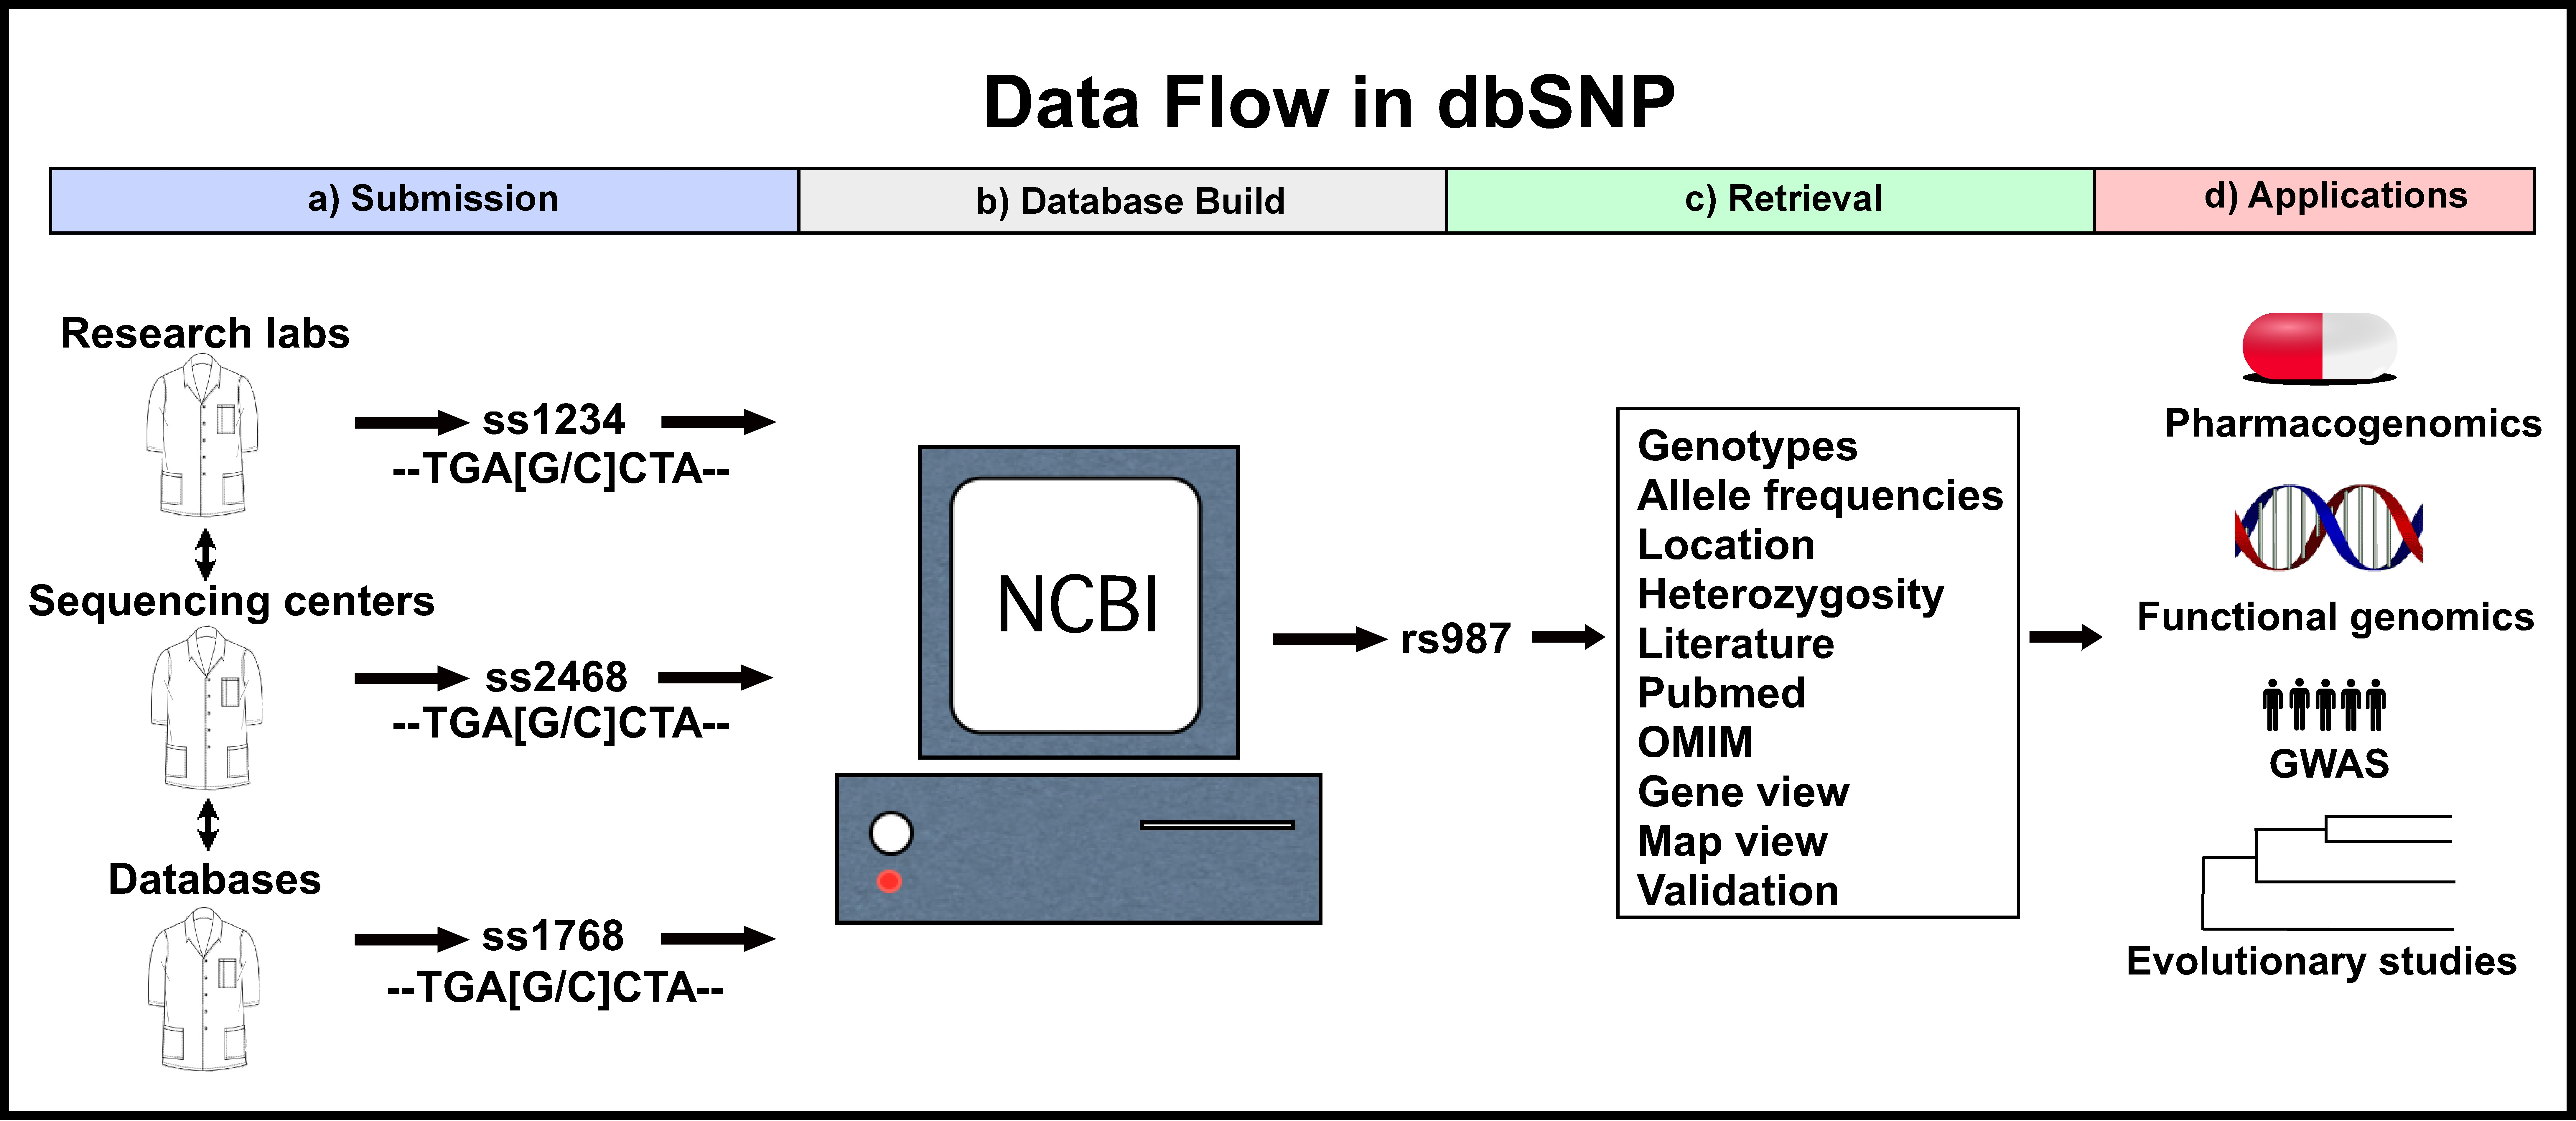
\includegraphics[width=0.7\textwidth]{./Graphics/DbSNP_diagram_no_caption.jpg}
	\caption{Initialisierung eines Bloomfilter Q vom 3 SNPs, k=3 Hashfunktionen und einem m=12 Bit langem Array }
	\label{fig:Bild2}
\end{figure}


\section{Anwendung}

Zwar wurde mit den in diesem Praktikum behandelten Algorithmen kein bestimmtes Ziel verfolgt, jedoch lassen sich diverse Anwendungsmöglichkeiten erdenken. 

\subsection{Personalisierte Medizin}

In der personalisierte Medizin werden individuelle Eigenschaften von Personen berücksichtigt um Therapien und Medikamente gezielt anzuwenden.
Hierzu können Therapien an bestimmte genetische Profile gekoppelt werden.

Um festzustellen, ob eine Therapie für einen Patienten zulässig ist, muss daher zunächst sein genetischer Code mit dem für diese Therapie notwendigem verglichen werden.
Derzeit werden diese Vergleiche ohne die entsprechenden Datensicherheits-Vorkehrungen vorgenommen.
Ziel dieses Praktikums war es durch Anwendung der genannten Methoden die Sicherung der Privatsphäre bei der Durchführung eines solchen Vergleichs zu erhöhen.

Jede Person besitzt eine einzigartige Version des menschlichen Genomes. Die allermeisten Variation zwischen einzelnen Personen haben keine Effekt auf die Gesundheit des Individuums. Jedoch gibt es einige wenige, welche Einfluss auf den Verlauf der Krankheit sowie auf die Wirksamkeit eines Verwendeten Medikamentes besitzen. 

Genau dies macht sich die personalisierte Medizin zunutze. 
Hier sind Therapien bestimmte genetische Marker gekoppelt.
Hierbei kann es sich unter anderem um SNP Profile handeln.
Diese werden erstellt indem der genetische 
Um festzustellen, ob eine Therapie für einen Patienten zulässig ist, müssen daher zunächst die Individuellen Variationen des Patienten mit denen für diese Therapie sinnvollen verglichen werden.


\section{Next generation sequencing}
In den ersten Jahren des 21.Jahrhunderts wurden mehrere Sequenzierungstechnicken entwickelt, welche unter dem Begriff next generation sequencing (NGS) zusammengefasst werden.
Sie alle vereint die Fähigkeit, DNA in großem Maßstab parallel sequenzieren zu können. 
Dies hatte zur Folge, dass NGS Sequenzierungen im Vergleich zur klassischen Sanger Sequenzierungen in den darauf folgenden Jahren deutlich schneller und günstiger wurden.
Kostete die Sequenzierung eines Genoms 2000 noch über 10 Millionen US Dollar, sind die Preise bis zum heutigen Tag auf unter 1000 gefallen.
  



